\begin{abstract}
 The abstract goes here...
\end{abstract}




%*****************************************
\chapter{Introduction}
%*****************************************
\hint{This chapter should motivate the thesis, provide a clear description of the problem to be solved, and describe the major contributions of this thesis. The chapter should have a length of about two pages!}

\section{Motivation}
What is the motivation for doing research in this area?

\section{Problem Statement and Contribution}
What is the problem that should be solved with this thesis?

\section{Outline}
How is the rest of this thesis structured?



%*****************************************
\chapter{Background}
\label{ch:background}
%*****************************************
\hint{This chapter should give a comprehensive overview on the background necessary to understand the thesis.
The chapter should have a length of about five pages!}


\section{Basics of Neural Networks\ \ \  \(WIP\)}
Neural networks are a part of most major AI-breakthrough in the last decade enabling computers to compete in fields formerly championed by humans.\footnote{
	\begin{itemize}
		\item 
			2011: "Watson" of IBM defeats two former grand champions in "Jeopardy!" \cite{lally2011natural}
		\item 
			2011: "Siri" enables users to use natural language to interact with their phones 
			\cite{ARON201124}
		\item 
			2015: A convolutional neural network classifies images from the ImageNet dataset more accurately than human experts 
			\cite{Russakovsky2015} \cite{He_2015_ICCV}
		\item 
			2016: "AlphaGo" beats Lee Sedol, one of the world's strongest Go players
			\cite{gibney2016google} \cite{silver2017mastering}
	\end{itemize}
}
They implement a statistical understanding of AI, which is to say that they try to find a specific model optimizing the likelihood of reproducing input-output pairs similar to some training data. The competing philosophy directly divines behaviour rules, frequently from expert knowledge, and as such is far less dependant from data.  
\textcolor{red}{[citation needed]}\\
For the former concept its model classes are the essential point of design. A multitude of properties maybe sought after in a model class of which a few important ones are:
\begin{itemize}
	\item \textbf{Richness:}\\
	The diversity of single models in the class and thus the ability to fit a wide field of different input-output landscapes.\footnote{
		More formally the richness of a model class can be described as the amount of different functions from the input-space to the output-space which can be expressed through a model of said class.}\\
	If a model class is inherently restricted the underlying relation between inputs and outputs might simply be beyond the expressive capabilities of all its models.\\
	In other words: If a model class is not rich enough all of its models will underfit the given training data.
	\item \textbf{Stability:}\\ 
	Tendency of similar models in the class to handle inputs in a similar way.\\
	If your model class shows unstable behavior defining a sensible way to search it for good models becomes difficult.
	\item \textbf{Interpretability of Models:}\\
	 Ease of formulating knowledge out of any given model in the class.\\
	 As fields exist in which statistical AI outperform experts the extraction of knowledge understandable and applicable by humans naturally is of interest.
	\item \textcolor{red}
	{[citation needed]}
\end{itemize}
If one knows an entity that already performs well on a given task it is a sensible approach to design ones model class to reproduce its decision process. Humans usually are such entities for many tasks of interest to AI research so they are a natural source of inspiration. Neural networks essentially are simplified models of a human central nervous system. \\
The most basic building block of the human central nervous system is a neuron which can receive multiple stimuli and is able to produce an output if the combined stimulation exceeds a threshold.\textcolor{red}{[citation needed]} One such neuron and its stimulus measure are depicted in Figure [\ref{fig:neuron1}]. Another functionality observed in nature is the ability of a neuron to strengthen the connection to any source of stimulus thus giving said source more influence on whether the neuron produces an output. 
\textcolor{red}{[citation needed]}\\
\\
The canonical mathematical model a neuron is defined as:
\begin{itemize}
	\item \textbf{Inputs} $x_i$ \textbf{:}\\
	All stimuli of a neuron are simply referred to as its inputs
	\item \textbf{Weights} $w_i$ \textbf{:}\\
	The ability to assign importances is modelled as weights which are coupled to specific stimuli
	\item \textbf{Combined Weighted Inputs} $\sum_{i=1}^{n}w_i x_i$ \textbf{:}\\
	After the inputs are scaled by their according weight they superpose to form the total excitation of the neuron
	\item \textbf{Activation Function} $\Phi(\sum_{i=1}^{n}w_i x_i)$ \textbf{:}\\
	
	\item \textbf{Bias} $b$ \textbf{:}\\  
	As the threshold is implicitly modelled in the activation function...
\end{itemize}
seen in Figure \ref{fig:neuron2} \\


\begin{figure}
	\centering
	\begin{minipage}{0.45\textwidth}
		\centering
		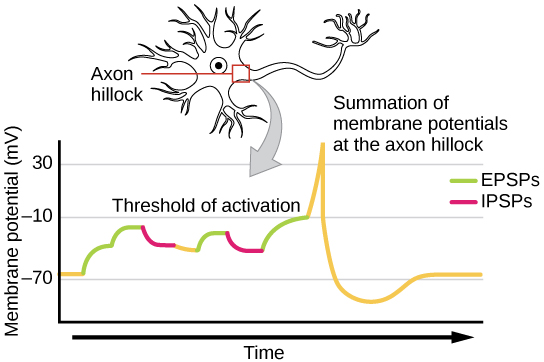
\includegraphics[height=150px]{gfx/Biological_Neuron.jpg}
		\caption{Representation of a biological Neuron}
		\label{fig:neuron1}
	\end{minipage}\hfill
	\begin{minipage}{0.45\textwidth}
		\centering
		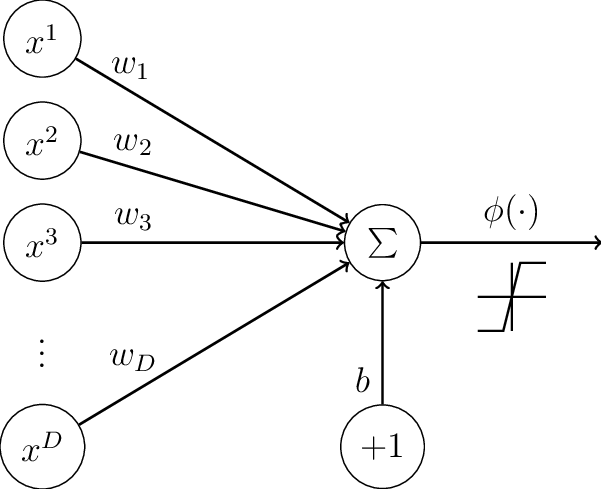
\includegraphics[height=150px]{gfx/Abstract_Neuron.png}
		\caption{Abstraction of a Neuron}
		\label{fig:neuron2}
	\end{minipage}
\end{figure}

As the individual neurons is too simple to model any complex relation between inputs
and outputs the next step is to aggregate multiple neurons. Figure \ref{fig:FFNetwork} displays a few neurons coming together to form a simple fully-connected feed-forward network.
\footnote{
	Inputs of neural networks are often called "features" and fully-connected networks are frequently referred to as "dense"	}
\begin{figure}
	\centering
		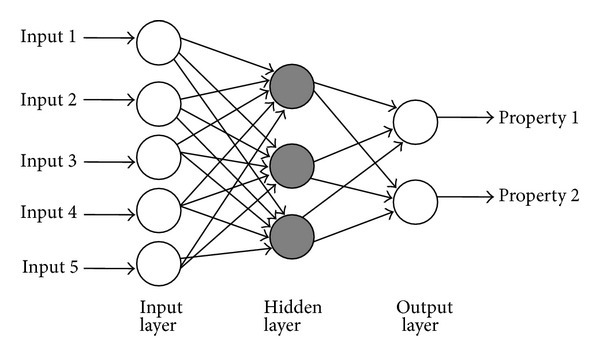
\includegraphics[height=150px]{gfx/Dense_FFNetwork.jpg}
		\caption{A small fully-connected network}
		\label{fig:FFNetwork}
\end{figure}

\begin{itemize}
	\item \textcolor{red}{TODO:}
	\item Issue of computational expense
	\item CNNs (and other forms of NN?)
\end{itemize}
	
\section{The Lottery Ticket Hypothesis}
\begin{itemize}
	\item \textcolor{red}{TODO:}
	\item Issue of overloading on parameters
	\item Clarifying the task (image classification)
	\item Idea of trainable subnets
\end{itemize}

\section{Basics of Natural Language Processing}
\begin{itemize}
	\item \textcolor{red}{TODO:}
	\item (?) Corpora
	\item Tokenizing
	\item Language Models
\end{itemize}

\section{Combining LMs \& CNNs}
\begin{itemize}
	\item \textcolor{red}{TODO:}
	\item Interpreting the tensor representation of a sentence/document as an image to be classified
	\item (?) Validation through results
	\item (?) Handeling different sizes of inputs
	\item (?) Handeling missing words in the Language model
\end{itemize}


%*****************************************
\chapter{Related Work}
\label{ch:relatedwork}
%*****************************************
\hint{This chapter should give a comprehensive overview on the related work done by other authors followed by an analysis why the existing related work is not capable of solving the problem described in the introduction.
The chapter should have a length of about three to five pages!}
\section{Lottery-Ticket-Hypothesis}
\begin{itemize}
	\item \textcolor{red}{TODO:}
	\item Emergence of safe "return points" after a few training epochs
	\item Ablation study
\end{itemize}

\section{Related Work Dynamic Pruning}

\section{Related Work Network Architecture Search}

\section{Analysis of Related Work}

\section{Summary}

%*****************************************
\chapter{Design}
\label{ch:design}
%*****************************************
\hint{This chapter should describe the design of the own approach on a conceptional level without mentioning the implementation details. The section should have a length of about five pages.}

\section{Requirements and Assumptions}

\section{System Overview}

\subsection{Component 1}

\subsection{Component 2}

\section{Summary}

%*****************************************
\chapter{Implementation}
\label{ch:implementation}
%*****************************************

\hint{This chapter should describe the details of the implementation addressing the following questions: \\ \\
1. What are the design decisions made? \\
2. What is the environment the approach is developed in? \\
3. How are components mapped to classes of the source code? \\
4. How do the components interact with each other?  \\
5. What are limitations of the implementation? \\ \\
The section should have a length of about five pages.}
\section{Design Decisions}

\section{Architecture}

\section{Interaction of Components}

\section{Summary}

%*****************************************
\chapter{Evaluation}
\label{ch:evaluation}
%*****************************************
\hint{This chapter should describe how the evaluation of the implemented mechanism was done. \\ \\
1. Which evaluation method is used and why? Simulations, prototype? \\
2. What is the goal of the evaluation? Comparison? Proof of concept? \\
3. Wich metrics are used for characterizing the performance, costs, fairness, and efficiency of the system?\\
4. What are the parameter settings used in the evaluation and why? If possible always justify why a certain threshold has been chose for a particular parameter.  \\
5. What is the outcome of the evaluation? \\ \\
The section should have a length of about five to ten pages.}
\section{Goal and Methodology}

\section{Evaluation Setup}

\section{Evaluation Results}

\section{Analysis of Results}


%*****************************************
\chapter{Conclusions}
\label{ch:closure}
%*****************************************

\hint{This chapter should summarize the thesis and describe the main contributions of the thesis. Subsequently, it should describe possible future work in the context of the thesis. What are limitations of the developed solutions? Which things can be improved?
The section should have a length of about three pages.}

\section{Summary}

\section{Contributions}

\section{Future Work}

\section{Final Remarks}
